\documentclass[12pt,a4paper,twoside]{article}
\usepackage[T1]{fontenc}
\usepackage[utf8]{inputenc}
\usepackage{indentfirst}
\usepackage{fancyhdr}
\usepackage{hyperref}
\usepackage{graphicx}
\usepackage{hyperref}
\usepackage{color}


\begin{document}

\title {\textbf {\color {blue} Le Mans Université}\color{black}
\\Licence Informatique  
\\ \textit {2éme année}
\\ \textbf {\color {red}EraDUCKation}
\author{Vaidie Camille, Philippe Marion,Marchand Killian,Touze Maxime}
\\ Version : 1.2 
\date \today }
\maketitle 
\begin {figure}
\begin{center}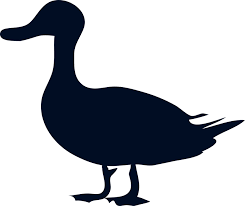
\includegraphics[width=0.15\textwidth]{images.png} \end{center}
\hspace{100pt}
\end {figure}
\newpage
\tableofcontents
\newpage
\section{Introduction}
    Ce rapport de projet traite du jeu EraDUCKation. Le jeu est inspiré par l'un des énoncés proposés :
 \textit{la vie dans un labyrinthe}, qui consiste à générer automatiquement
 un labyrinthe dans lequel des insectes doivent évoluer. Les règles sont 
simples: la reproduction est similaire au \textit{jeu de la vie} vu en cours, il faut intégrer des déplacements semi-aléatoires pour 
les insectes, ainsi qu'une notion de nourriture et des statistiques sur 
la population.
\\
\\Cependant, comme pour le \textit{jeu de la vie} vu en cours, nous
trouvons que ce projet a trop peu d'interaction, et avons donc décidé 
d'en faire un jeu. Nous préférons passer sur des canards par pur intérêts 
personnels, c'est un moyen de mettre une touche personnelle dans notre projet, 
nous sommes donc passé d’un programme à un jeu plus interactif.
\\
\\Nous avons donc créer un jeu basé sur \textit{la vie dans un labyrinthe} en modifiant les condition d'accouplement, en intégrant des déplacements se basant sur la vue (ou non) d'un partenaire, de reproduction ou de nourriture. Nous avons créer un mode solo, un multijoueur sur un même écran et un multijoueur en réseau LAN. Ainsi que trois modes de difficultés : 
facile, intermédiaire et difficile. Le programme doit aussi disposer d'une interface graphique. \\
\\Le principe du jeu est simple, vous êtes un dieu et vous devez sélectionner des événements qui influeront sur la vie des canards qui sont prisonniers d’un labyrinthe. Le but est de faire survivre une colonie de canards durant 100 générations et de faire le plus gros score. Pour cela nous jouons avec des événements qui seront là pour nous aider ou nous bloquer.\\
\newpage
\section{Organisation du travail}
Pour organiser notre travail nous avons en premier lieu mis en place un Google drive qui sert de carnet de bord avec toutes nos idées, notre organisation, et ce que l'on comptait faire lors de chaque séance.\\
On a mis en place un Github dès la première séance qui a servi tout au long du projet pour garder et partager tous nos codes.
\\On a donc dès la première séance décidé de se répartir les tâches en fonction des envies et aptitudes de chacun. On a aussi décidé de celles qui seraient obligatoires pour notre projet et celles qui seraient optionnelles. Ce qui nous a amené à cette organisation prevu :
Ainsi ce qui est présent en orange est optionnel, le reste obligatoire. \\
\begin {figure}[h]
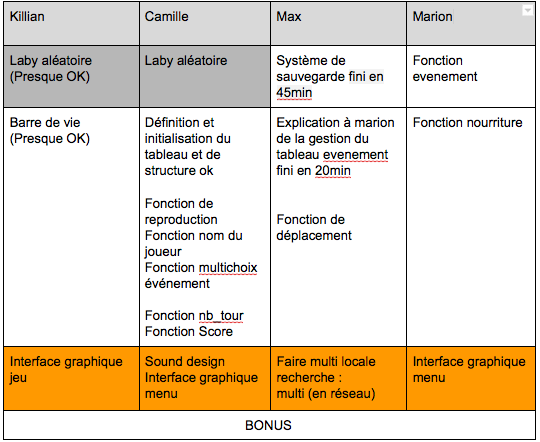
\includegraphics[width=1\textwidth]{prevision.png}
\caption{\label {ref2}Organisation prévue au début du projet}
\end {figure}

Ensuite, nous avons commencé les recherches et le code dès la première séance.
On a donc passé les trois premières séances à coder toutes les fonctions du jeu en lui même (événements, joueur, déplacement, nourriture, etc). Ainsi que le labyrinthe et son affichage en caractères ISO.
Puis, après des recherches, on a codé le labyrinthe en unicode.
\\
\\
On a commencé le jeu en solo puis en multijoueur local. On a aussi dès la cinquième séance commencé les recherches concernant la SDL et ce qu'on pourrait faire avec notre jeu. Ensuite on a passé la fin du projet à déboguer nos codes, à tester nos erreurs, améliorer nos codes ainsi que le jeu.
\begin {figure}[h]
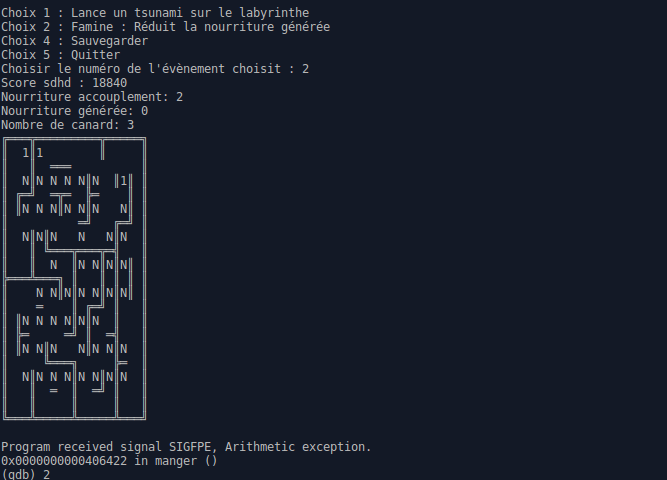
\includegraphics[width=0.3\textwidth]{debbeug.png}
\hspace{100pt}
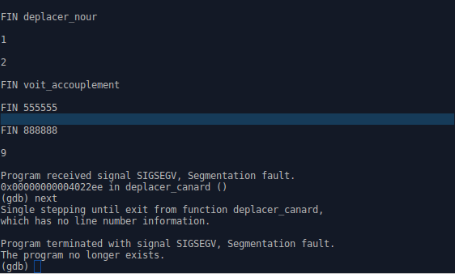
\includegraphics[width=0.3\textwidth]{debug.png}
\caption{\label {ref3}débogage}
\end {figure}
\\
\\
Puis on a continué à développer le multijoueur local et en réseau.
En conclusion notre organisation finale du projet a été la suivante :
\begin {figure}[h]
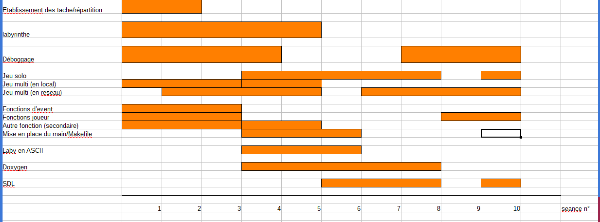
\includegraphics[width=1.1\textwidth]{grantt.png}
\caption{\label {ref4}Organisation réelle du projet}
\end {figure}
Et a une répartition finale plutot équilibré entre chaque membre du groupe : \\
\begin {figure}[h]
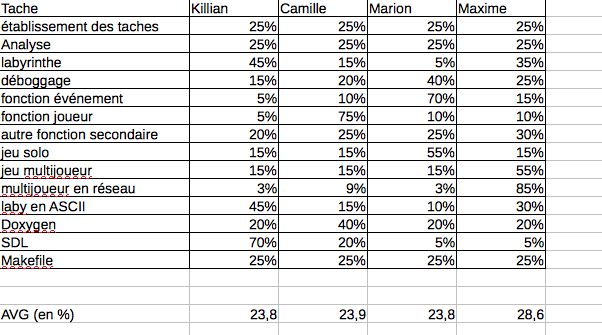
\includegraphics[width=1.1\textwidth]{pourc.png}
\caption{\label {ref4}répartition réelle du projet}
\end {figure}
\newpage
\section{Analyse - Comment jouer ?}

Dans « EraDUCKation », il y a deux types de jeu.
\\
On a d'abord un mode solo, puis un mode multijoueur en local ou en réseau. 
\\
Dans le mode solo, comme dans le multijoueur, le joueur effectue des choix via les touches « 1,2,3 » du clavier.
\\
On a la possibilité de faire des choix dans deux catégories:
\begin{enumerate}
\item- Les bons événements
\begin{enumerate}
\item- boost de la reproduction des canards
\item- boost de nourriture
\item- invisibilité d'un canard
\item- libération de canards
\item- rien faire
\end{enumerate}
\item- Les mauvais événements
\begin{enumerate}
\item- tsunami
\item- tempête
\item- famine
\item- reproduction ralentie
\item- apparition d'un prédateur
\end{enumerate}
\end{enumerate}
\begin{figure}[h]
\centering
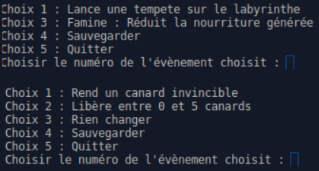
\includegraphics[width=0.6\textwidth]{event.png}
\caption{Exemple de bons et mauvais événements.}
\end{figure}
Comme vu dans les règles en solo le joueur utilise des événements bon et mauvais,
c'est à lui de faire les bons choix afin de faire survivre sa communauté sous la contrainte des mauvais événements.
\\ \\
Contrairement au solo, le multijoueur permet aux joueurs de choisir leur rôle (ils ont le choix d'être le bon ou le mauvais dieu), et donc de se battre pour la survie, ou non, de la colonie.
\\ \\
Le joueur à la possibilité de choisir son pseudo en début de partie, tant en solo qu'en multijoueur.
\\ \\
Un système de sauvegarde est mis au point afin de donner la possibilité au joueur de quitter sa partie en cours, et de pouvoir reprendre sa partie ultérieurement en choisissant dans le menu l'option « charger partie ».
\\ \\
Dans les deux modes de jeu, on attribue aux joueurs un score qui évolue en fonction des actions qu’ils font.
Par exemple en solo, le joueur gagne des points s’il arrive à faire ce qu'il faut pour la survie des canards mais perd des points s’il en tue.
\\ \\
En multijoueur, l’attribution des points est différents puisque quand un joueur fait une action il gagne un certain nombres de points, tandis que son adversaires perd ce même nombre de points. Le but est donc de finir la partie avec le meilleur score. Et cela dépend de la rapidité du mauvais dieu à exterminer la colonie de canard.
\newpage
\section{Conception}
Le programme permet le déplacement, de faire apparaître de la nourriture ou de générer un labyrinthe aléatoirement. Il permet aussi de gérer les événements que le joueur choisi durant la partie. 
\\Par exemple un Tsunami peut tuer un certain nombre de canards, si ces derniers sont sur la trajectoire de l'événement.D’un point de vu programmation, le tsunami traverse une ligne de la matrice choisie aléatoirement, si un ou plusieurs canard sont sur cette même ligne, ils meurent.
\\L'événement “boost de nourriture” augmente le nombre de nourriture à générer dans le labyrinthe.
Il permet aussi de gérer un mode de jeu solo, mais aussi multijoueur.
\\Le multijoueur se décompose en deux modes : le mode local consiste à jouer à deux joueurs sur le même écran, et le mode réseau permet à deux joueurs de jouer chacun sur son écran.
\subsection{Labyrinthe aléatoire}
\begin{figure}[h]
\centering
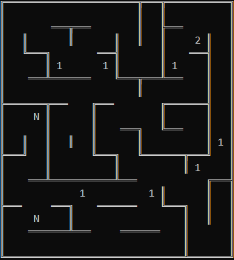
\includegraphics[width=0.6\textwidth]{laby_dern.png}
\caption{labyrinthe généré aléatoirement en difficulté facile}
\end{figure}
\newpage
La mise en place du labyrinthe aléatoire permet d'instaurer une rejouabilité et une expérience de jeu différente à chaques parties. Mais aussi de rajouter un côté surprenant au jeu, c'est-à-dire, que l'on peut très bien commencer une partie et avoir un labyrinthe très simple comme tomber à la partie suivante sur un labyrinthe avec plus de mur, et donc plus complexe.
\subsection{Le multijoueur}
Le multijoueur apporte un plus au jeu. Tout comme le labyrinthe aléatoire, le multi
apporte une nouvelle façon de jouer à EraDUCKation. En effet sur un tour, le premier joueur est le “bon” dieu (ici joueur : killian) et il a le choix entre des événements favorable à ses canards. Alors que deuxième joueur (ici camille), est le “mauvais” dieu, et à lui le choix entre des événements défavorables aux canards.
\begin{figure}[h]
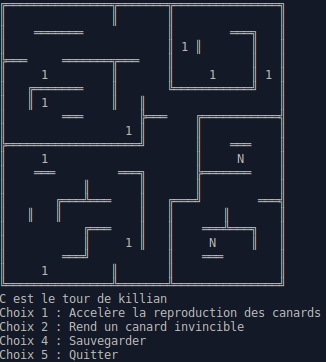
\includegraphics[width=0.5\textwidth]{tour_kiki.png}
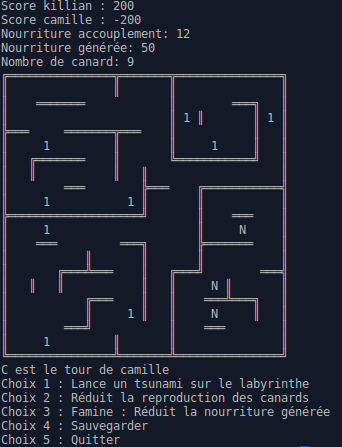
\includegraphics[width=0.5\textwidth]{tour_cam.png}
\caption{Tour en multi (bon et mauvais dieu}
\end{figure}
Nous avons aussi commencé un multijoueur en réseau qui utilise ce protocole de communication en réseau.
\begin{figure}[h]
\centering
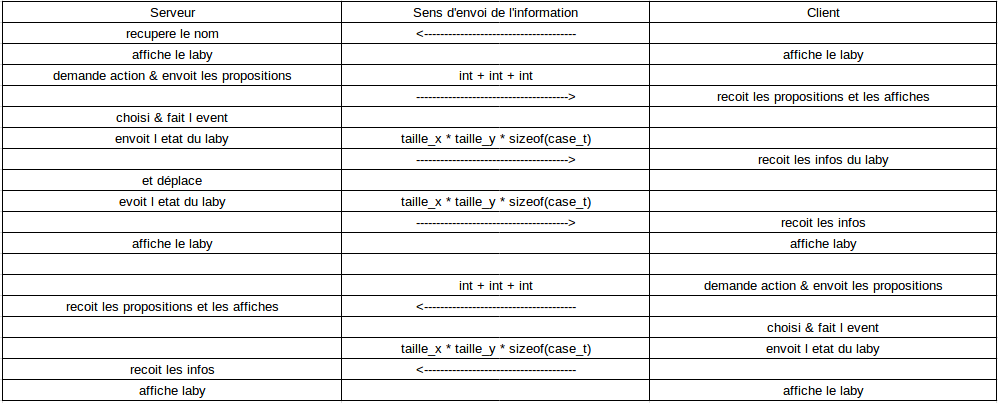
\includegraphics[width=0.8\textwidth]{reseau.png}
\caption{protocole de communication}
\end{figure}
\newpage
\section{Programmation}
\subsection{Programmation modulaire}
EraDUCKation contient différents types de modules : des modules liés au contenu du jeu lui-même (module canard, piège, nourriture, déplacer, structure, reproduction, matrice, joueur, événement), des modules liés à des fonctionnalités (sauvegarde, multijoueur joueur local et réseau, connexion) et enfin des modules boîtes à outils.
\begin{figure}[h]
\centering
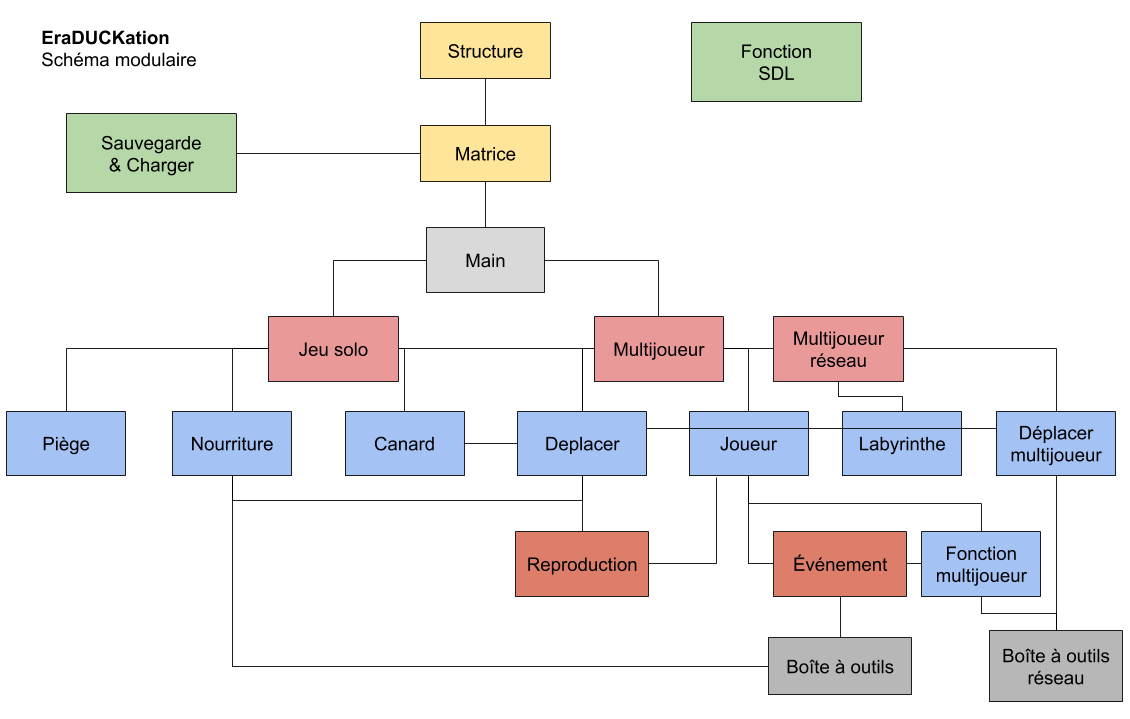
\includegraphics[width=1\textwidth]{module.png}
\caption{Schéma modulaire}
\end{figure}
\subsection{Labyrinthe}
La création de notre jeu commence par la création du labyrinthe. On définit donc une matrice pour notre labyrinthe et la taille de cette dernière varie en fonction de la difficulté choisie au lancement du jeu.
\\
\\
Le labyrinthe est défini par une matrice où chaque case contient 4 murs (Nord, Sud, Est, Ouest) et une valeur qui servira pour la création des différentes galeries du labyrinthe. L’algorithme consiste à remplir la matrice avec tous les murs possible et ensuite à les détruire aléatoirement. C’est donc là qu’intervient la valeur de la case, puisque à chaque nouvelle création de galeries dans le labyrinthe cette valeur est incrémentée. 
\\Une fois que ça fait une seule et unique galerie le programme s’arrête. Pour cela, il va comparer les galeries adjacentes et va déterminer la valeur minimum, puis casser un mur pour joindre les galeries.Enfin toutes les cases de la nouvelle galerie prendront la valeur minimum des deux anciennes galeries.\\
Cet algorithme contient de nombreuses vérifications : mise en place des coins du labyrinthe, un nombre minimal de mur dans une case de la matrice pour qu’il ressemble à un vrai labyrinthe, la destruction d’un mur s’il existe déjà ce même mur dans une case adjacente. 
\\Pour éviter de compliquer la matrice déjà existante nous avons préféré mettre en place une matrice interne à la création du labyrinthe et ensuite la copier dans la matrice utilisée dans tous les autres programmes.\\
Pour ce qui est de l’affichage, nous avons d’abord utilisé pour la vérification du bon fonctionnement de l’algorithme, un affichage basique, où l’on affichait simplement l’état de chaque case sous forme de tableau à l’écran.\\
\begin{figure}[h]
\centering
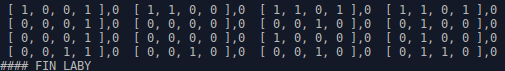
\includegraphics[width=1\textwidth]{laby_prem.png}
\caption{Première version du laby}
\end{figure}
\\
Dans un second temps, nous avons affiché le labyrinthe avec des caractères simple du clavier. Principalement des espaces, des "$|$" ou encore "\_".\\
\begin{figure}[h]
\centering
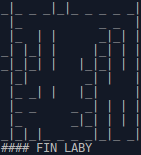
\includegraphics[width=0.3\textwidth]{laby_deux.png}
\caption{Seconde version du laby}
\end{figure}
\\
\\
Enfin nous arriver à créer une fonction d’affichage, qui nous permet d’afficher un labyrinthe propre à l’écran. C’est-à-dire qu’à l’aide de code unicode nous avons des bordures sans espace, ce qui permet d’avoir un labyrinthe fermé. \\
\begin{figure}[h]
\centering
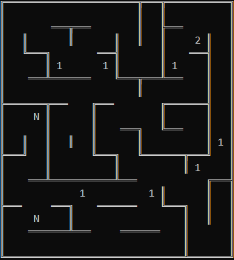
\includegraphics[width=0.4\textwidth]{laby_dern.png}
\caption{Dernière version du labyrinthe}
\end{figure}
\subsection{Déplacer}
La principale fonctionnalité liée aux canards est le déplacement qui contient un rapport avec la nourriture et les autres canards. Elle consiste à faire déplacer une fois sur trois les canards adultes présents dans la matrice. Elle permet aussi de créer le comportement des canards, ils vont chercher à s’accoupler en priorité puis ensuite se nourrir. \\
\begin{figure}[h]
\centering
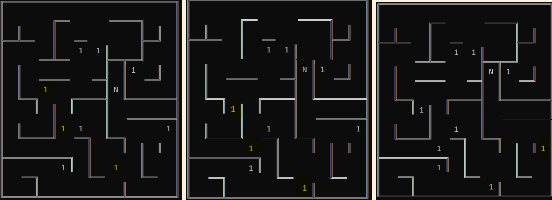
\includegraphics[width=0.8\textwidth]{deplacer.png}
\caption{Déplacement}
\end{figure}
\subsection{SDL}
Nous avons mis en place les bibliothèques SDL 2, SDL\_image et SDL\_ttf, afin de faire les 
graphismes du jeu. Pour cela nous avons dû, à partir d’un algorithme de création de fenêtre.
SDL, créer les différentes textures que nous avons besoin dans notre projet.
Notre interface graphique consiste essentiellement au menu de départ, composé de trois, bouton (Play, Credit, Quit).
En appuyant sur Play, rien ne se passe sur la fenêtre SDL, mais dans le terminal de l’ordinateur le jeu se lance.\\
\begin{figure}[h]
\centering
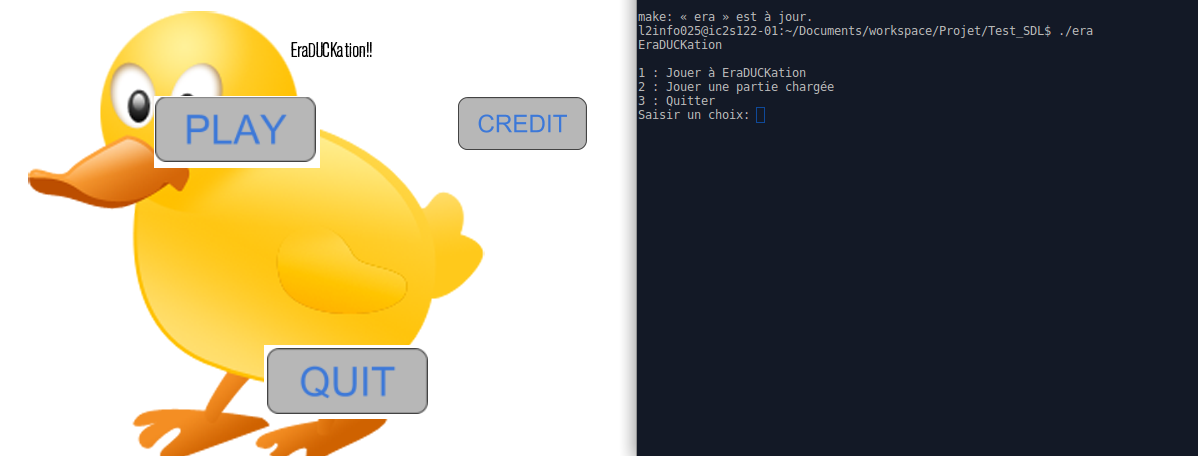
\includegraphics[width=1\textwidth]{jeu.png}
\caption{Menu SDL : lancement du terminal}
\end{figure}
\newpage
\section{Résultats}
    Nous sommes parvenus à remplir toutes les fonctionnalités imposées,
telles que la sauvegarde, et donc le chargement d’une partie, mais aussi la
génération aléatoire d'un labyrinthe, le jeu en mode solo et en multi-joueurs,
les évènements aléatoires (même si le joueur choisi, il choisit entre des
évènements aléatoires), la gestion de nourriture, notre propre système de
reproduction basé sur la nourriture que possède un canard, un déplacement priorisant
la reproduction, puis la nourriture si le canard en a besoin, ou si il ne voit rien,
une décision aléatoire.
\\Nous avons rajouté en plus des fonctionnalités obligatoires le jeu en multijoueur réseau et un début d’interface graphique. 
\subsection{Fonctionnalités obligatoires}
\subsubsection{Sauvegarde et chargement}
    La sauvegarde et le chargement des parties sont censés fonctionner. Cependant ils créent une segmentation fault que nous n’avons pas eu le temps d’identifier. 
\subsubsection{Génération du labyrinthe}
    La génération de labyrinthe est aléatoire et fonctionnelle. Chaque case a au minimum deux murs, sauf exception (qui évite une boucle infinie lors d’une création d’un labyrinthe impossible à résoudre avec cette condition), et les cases sont toutes reliées entre elles. 
\subsubsection{Jeu solo et multijoueur, et leurs fonctionnalités }
    Les modes de jeux solos et multijoueurs sont tout à fait opérationnels, à l’exception d’une fonctionnalité du multijoueur, l’ordre de jeu, que nous avons voulus implémenter, mais à cause d’erreurs non trouvées nous avons dû le laisser de côté. Le reste fonctionne cependant parfaitement, chaque événement agit comme il doit le faire. Les déplacements n’ont pas le moindre effet de bord et réagissent correctement à l'environnement (reproduction possible, vue sur la nourriture…), la génération de nourriture se fait comme elle le doit, tout comme la reproduction. Les canards arrivent dans le labyrinthe en tant que oeufs, et deviennent des adultes à la génération suivante
\subsection{Fonctionnalités facultatives}
\subsubsection{Jeu en réseau}
    Le mode de jeu en réseau ne compile pas, malgré les recherches nous ne trouvons pas l’erreur indiquée par le compilateur.
\subsubsection{Interface graphique}
    L’interface graphique dispose d’un menu fonctionnel. Cependant, par manque de temps, l’interface graphique n’est pas complète.
\section{Bilans personnels}
Concernant notre bilan personnel, il y a eu d’importantes révisions et amélioration sur certains points : 
\begin{enumerate}
\item- pointeur sur un tableau
\item- utilisation de pointeur en générale
\item- commenter nos codes
\item- création d’algorithme important
\item- l’amélioration du travail de groupe
\item- l’organisation prévisionnelle d’un projet
\item- l’organisation en groupe 
\end{enumerate}
Nous avons aussi de nouvelles notions comme : 
\begin{enumerate}
\item- SDL2  (graphisme du jeu)
\item- Socket et protocole : “chemin entre deux ordinateur”
\item- Création d’un labyrinthe aléatoire : gérer les effets de bords,logique de construction,...
\item- Organisation modulaire
\end{enumerate}
Nous avons aussi compris l’importance d’utilisation du débogueur et non du débogage “à la main”, ainsi que l’utilisation de programme de test, que nous n’avons pas réussi à mettre en place par manque de temps.
\\
\\
Nous avons réalisé ce projet en tant que projet de fin de seconde année de licence informatique mais aussi afin de le présenter lors d'une soutenance.
\end{document}
